\documentclass{jsarticle}
\usepackage{amsmath}
\usepackage{amssymb}
\usepackage{ascmac}
\usepackage{bm}
\usepackage{graphicx}

\flushbottom
\sloppy

\setlength{\paperwidth}{210mm}
\setlength{\paperheight}{297mm}
\setlength{\voffset}{0mm}
\setlength{\textwidth}{\paperwidth}
\addtolength{\textwidth}{-30mm}
\setlength{\textheight}{\paperheight}
\addtolength{\textheight}{-50mm}
\setlength{\topmargin}{-1in}
\addtolength{\topmargin}{20mm}
\setlength{\headheight}{0mm}
\setlength{\headsep}{0mm}
\setlength{\footskip}{20mm}
\setlength{\oddsidemargin}{-1in}
\addtolength{\oddsidemargin}{15mm}
\setlength{\columnsep}{7mm}

\title{\Large {\bf 合成剛体法(Composite Rigid Body Method)によるリンク系の慣性行列計算}}
\author{杉原知道}

\begin{document}
\maketitle

\section{まえがき}

リンク系運動方程式における慣性行列の計算方法は幾つか知られていますが,
代表的なのは
「{\bf 単位ベクトル法(unit vector method)}」
「{\b 合成剛体法(composite rigid body method)}」の二つでしょう.
これらはいずれもWalker and Orinにより示されたものです.
\begin{quote}
M. W. Walker and D. E. Orin,
Efficient Dynamic Computer Simulation of Robotic Mechanisms,
Transactions of the ASME, Journal of Dynamic Systems, Measurement, and Control,
Vol. 104, pp. 205--211, 1982.
\end{quote}
単位ベクトル法は分かりやすいので大抵のロボットの教科書で説明されています.
一方,合成剛体法は単位ベクトル法よりも高速で実用的なのですが,
説明している教科書はなぜかほとんどありません.
筆者の所有する書籍では,次のFeatherstoneにしか書いてありませんでした.
\begin{quote}
R. Featherstone,
Robot Dynamics Algorithms,
Kluwer Academic Publishers, Boston/Dordrecht/Lancaster, 1987.
\end{quote}
Featherstoneの空間ベクトル表現は表記を簡単にしますが,
計算効率の良い実装をするには中身を知っている必要があります.
このような事情から本記事を書くことにしました.
剛体リンク系の運動方程式についてある程度知識を持っている読者を想定しています.


\section{リンク系慣性行列に関する数学的準備}

リンク系の運動方程式は,一般的に次の形で表せます.
\begin{align*}
\bm{H}(\bm{q})\ddot{\bm{q}}+\bm{b}(\bm{q},\dot{\bm{q}})=\bm{\tau}+\bm{J}(\bm{q})^{\mathrm{T}}\bm{f}
\end{align*}
ただし,
$\bm{q}$は一般化座標,
$\bm{H}(\bm{q})$は慣性行列,
$\bm{b}(\bm{q},\dot{\bm{q}})$はバイアス力(遠心力・コリオリ力・重力をまとめたもの),
$\bm{\tau}$は一般化座標に対応する一般化力,
$\bm{f}$は外力,
$\bm{J}(\bm{q})$は外力の作用する接触点のヤコビ行列
です.
リンク系は,分岐はあるがループは持たない開構造であるものとします.
本記事の関心事項は慣性行列$\bm{H}(\bm{q})$のみなので,
無重量空間でリンク系が速度を持たず(つまり$\bm{b}(\bm{q},\dot{\bm{q}})=\bm{0}$),
外力も作用していない($\bm{f}=\bm{0}$)世界での運動を考えれば十分です.
\begin{align*}
\bm{H}(\bm{q})\ddot{\bm{q}}=\bm{\tau}
\end{align*}

さて,慣性行列の中身は次のようになっています.
\begin{align*}
\bm{H}(\bm{q})=\sum_{i=1}^{n}\left(
m_{i}\bm{J}_{\mathrm{G}i}(\bm{q})^{\mathrm{T}}\bm{J}_{\mathrm{G}i}(\bm{q})
+\bm{J}_{\mathrm{A}i}(\bm{q})^{\mathrm{T}}\bm{I}_{i}(\bm{q})\bm{J}_{\mathrm{A}i}(\bm{q})
\right)
\end{align*}
ただし,
$n$は全リンク数,
$m_{i}$は$i$番目リンクの質量,
$\bm{I}_{i}(\bm{q})$は$i$番目リンクの重心まわり慣性テンソル
で,
$i$番目リンクの姿勢行列を$\bm{R}_{i}(\bm{q})$,
リンク座標系における重心まわり慣性テンソル(定数行列)を${}^{i}\bm{I}_{i}$とそれぞれおけば,
\begin{align*}
\bm{I}_{i}(\bm{q})=\bm{R}_{i}(\bm{q}){}^{i}\bm{I}_{i}\bm{R}_{i}(\bm{q})^{\mathrm{T}}
\end{align*}
です.
また,
$\bm{J}_{\mathrm{G}i}(\bm{q})$と$\bm{J}_{\mathrm{A}i}(\bm{q})$は$i$番目リンクは次式を満たす行列です.
\begin{align*}
\dot{\bm{p}}_{\mathrm{G}i}=\bm{J}_{\mathrm{G}i}(\bm{q})\dot{\bm{q}}
\\
\bm{\omega}_{i}=\bm{J}_{\mathrm{A}i}(\bm{q})\dot{\bm{q}}
\end{align*}
ただし,
$\bm{p}_{\mathrm{G}i}$は$i$番目リンクの重心位置,
$\bm{\omega}_{i}$は$i$番目リンクの角速度
です.
重心を関心点とする基礎ヤコビ行列と呼んでも構いません.
ちなみにこの式の通りに計算を実装したときの計算量は,単位ベクトル法とあまり変わりません.
式から明らかに,$\bm{H}(\bm{q})$は対称行列かつ正定値行列となります.

一般化座標と一般化力は,
各リンクの関節変位$\bm{q}_{i}$と関節(駆動)力$\bm{\tau}_{i}$をまとめたものとして定められます.
\begin{align*}
\bm{q}=\left[\begin{array}{c}
\bm{q}_{0} \\
\bm{q}_{1} \\
\vdots \\
\bm{q}_{n}
\end{array}\right]
,\qquad
\bm{\tau}=\left[\begin{array}{c}
\bm{\tau}_{0} \\
\bm{\tau}_{1} \\
\vdots \\
\bm{\tau}_{n}
\end{array}\right]
\end{align*}
これに対応して,慣性行列は次のように分解できます.
\begin{align*}
\bm{H}(\bm{q})=\left[\begin{array}{cccc}
\bm{H}_{11}(\bm{q}) & \bm{H}_{12}(\bm{q}) & \cdots & \bm{H}_{1n}(\bm{q}) \\
\bm{H}_{12}(\bm{q})^{\mathrm{T}} & \bm{H}_{22}(\bm{q}) & \cdots & \bm{H}_{2n}(\bm{q}) \\
\vdots & \vdots & \ddots & \vdots \\
\bm{H}_{1n}(\bm{q})^{\mathrm{T}} & \bm{H}_{2n}(\bm{q})^{\mathrm{T}}& \cdots & \bm{H}_{nn}(\bm{q}) \\
\end{array}\right]
\end{align*}
つまり,
\begin{align*}
\left[\begin{array}{cccc}
\bm{H}_{11}(\bm{q}) & \bm{H}_{12}(\bm{q}) & \cdots & \bm{H}_{1n}(\bm{q}) \\
\bm{H}_{12}(\bm{q})^{\mathrm{T}} & \bm{H}_{22}(\bm{q}) & \cdots & \bm{H}_{2n}(\bm{q}) \\
\vdots & \vdots & \ddots & \vdots \\
\bm{H}_{1n}(\bm{q})^{\mathrm{T}} & \bm{H}_{2n}(\bm{q})^{\mathrm{T}}& \cdots & \bm{H}_{nn}(\bm{q}) \\
\end{array}\right]
\left[\begin{array}{c}
\ddot{\bm{q}}_{0} \\
\ddot{\bm{q}}_{1} \\
\vdots \\
\ddot{\bm{q}}_{n}
\end{array}\right]
=
\left[\begin{array}{c}
\bm{\tau}_{0} \\
\bm{\tau}_{1} \\
\vdots \\
\bm{\tau}_{n}
\end{array}\right]
\end{align*}
と書けるということです.

\section{合成剛体法}

\subsection{考え方}

運動方程式において,
仮想的に$i$番目関節以外の全ての関節の加速度がゼロである状況を考えましょう.
\begin{align*}
\left[\begin{array}{c}
\bm{H}_{1i}(\bm{q}) \\
\bm{H}_{2i}(\bm{q}) \\
\vdots \\
\bm{H}_{(i-1)i}(\bm{q}) \\
\bm{H}_{ii}(\bm{q}) \\
\bm{H}_{i(i+1)}(\bm{q})^{\mathrm{T}} \\
\vdots \\
\bm{H}_{in}(\bm{q})^{\mathrm{T}} \\
\end{array}\right]
\ddot{\bm{q}}_{i}
=
\left[\begin{array}{c}
\bm{\tau}_{0} \\
\bm{\tau}_{1} \\
\vdots \\
\bm{\tau}_{i-1} \\
\bm{\tau}_{i} \\
\bm{\tau}_{i+1} \\
\vdots \\
\bm{\tau}_{n}
\end{array}\right]
\end{align*}
$i$番目関節よりも先側のリンク群は一体となって運動します.
これを「$i$番目合成剛体」と呼ぶことにします.
$i$番目関節より根元側のリンク群は静止したままなので,$i$番目合成剛体の運動に影響しません.
$i$番目関節以外の関節には,
関節運動を拘束するための力(内力)が発生することになります.

$i$番目リンク座標系に対する
$i$番目合成剛体の質量,重心位置,慣性テンソルをそれぞれ
$m_{i}^{\mathrm{C}}$,
${}^{i}\bm{p}_{\mathrm{G}i}^{\mathrm{C}}$,
${}^{i}\bm{I}_{i}^{\mathrm{C}}$とおきましょう.
内力は全て打ち消し合うので,$i$番目関節に作用する6軸力${}^{i}\bm{f}_{i}$,${}^{i}\bm{n}_{i}$のみが
$i$番目合成剛体の運動を作ります.
これを記述する運動方程式は次式のようになります.
\begin{align*}
m_{i}^{\mathrm{C}}{}^{i}\hat{\bm{a}}_{\mathrm{G}i}^{\mathrm{C}}={}^{i}\bm{f}_{i}
\\
{}^{i}\bm{I}_{i}^{\mathrm{C}}{}^{i}\hat{\bm{\alpha}}_{i}={}^{i}\bm{n}_{i}-{}^{i}\bm{p}_{\mathrm{G}i}^{\mathrm{C}}\times{}^{i}\bm{f}_{i}
\end{align*}
ただし,
\begin{align*}
{}^{i}\hat{\bm{a}}_{\mathrm{G}i}^{\mathrm{C}}=\bm{R}_{i}^{\mathrm{T}}\ddot{\bm{p}}_{\mathrm{G}i}^{\mathrm{C}}
\\
{}^{i}\hat{\bm{\alpha}}_{i}=\bm{R}_{i}^{\mathrm{T}}\dot{\bm{\omega}}_{i}
\end{align*}
とおきました.
$\bm{\omega}_{i}$は$i$番目関節の運動により生じる合成剛体の角速度です.
仮想的に速度がゼロの状況を考えているので,$\bm{\omega}_{i}=\bm{0}$であることにご注意下さい
(このため遠心力・コリオリ力が生じません).
ここで
$i$番目リンク座標系原点位置を$\bm{p}_{i}$とおき,
\begin{align*}
{}^{i}\hat{\bm{a}}_{i}\overset{\mathrm{def}}{=}\bm{R}_{i}^{\mathrm{T}}\ddot{\bm{p}}_{i}
\end{align*}
を定義すれば,
\begin{align*}
\ddot{\bm{p}}_{\mathrm{G}i}^{\mathrm{C}}=\ddot{\bm{p}}_{i}-\bm{R}_{i}{}^{i}\bm{p}_{\mathrm{G}i}^{\mathrm{C}}\times{}^{i}\hat{\bm{\alpha}}_{i}
\quad\Leftrightarrow\quad
{}^{i}\hat{\bm{a}}_{\mathrm{G}i}^{\mathrm{C}}={}^{i}\hat{\bm{a}}_{i}-{}^{i}\bm{p}_{\mathrm{G}i}^{\mathrm{C}}\times{}^{i}\hat{\bm{\alpha}}_{i}
\end{align*}
です(ここでも向心加速度・コリオリの加速度が生じません).
これを運動方程式に代入し,行列を使ってまとめれば,
\begin{align*}
\left[\begin{array}{cc}
m_{i}^{\mathrm{C}}\bm{1} & -m_{i}^{\mathrm{C}}{}^{i}\bm{p}_{\mathrm{G}i}^{\mathrm{C}}\times \\
\bm{O} & {}^{i}\bm{I}_{i}^{\mathrm{C}}
\end{array}\right]
\left[\begin{array}{c}
{}^{i}\hat{\bm{a}}_{i}
\\
{}^{i}\hat{\bm{\alpha}}_{i}
\end{array}\right]
=
\left[\begin{array}{cc}
\bm{1} & \bm{O} \\
-{}^{i}\bm{p}_{\mathrm{G}i}^{\mathrm{C}}\times & \bm{1}
\end{array}\right]
\left[\begin{array}{c}
{}^{i}\bm{f}_{i}
\\
{}^{i}\bm{n}_{i}
\end{array}\right]
\\
\Leftrightarrow\qquad
\left[\begin{array}{cc}
m_{i}^{\mathrm{C}}\bm{1} & -m_{i}^{\mathrm{C}}{}^{i}\bm{p}_{\mathrm{G}i}^{\mathrm{C}}\times \\
m_{i}^{\mathrm{C}}{}^{i}\bm{p}_{\mathrm{G}i}^{\mathrm{C}}\times & {}^{i}\bm{I}_{i}^{\mathrm{C}}-m_{i}^{\mathrm{C}}{}^{i}\bm{p}_{\mathrm{G}i}^{\mathrm{C}}\times^{2}
\end{array}\right]
\left[\begin{array}{c}
{}^{i}\hat{\bm{a}}_{i}
\\
{}^{i}\hat{\bm{\alpha}}_{i}
\end{array}\right]
=
\left[\begin{array}{c}
{}^{i}\bm{f}_{i}
\\
{}^{i}\bm{n}_{i}
\end{array}\right]
\end{align*}
となります.
左辺の係数行列が合成剛体の慣性行列です.

根元側のリンク群は全て静止しているので,
$i$番目関節の加速度は次の様に関節加速度のみで表せます.
\begin{align*}
\left[\begin{array}{c}
{}^{i}\hat{\bm{a}}_{i}
\\
{}^{i}\hat{\bm{\alpha}}_{i}
\end{array}\right]
=
\left[\begin{array}{c}
{}^{i}\hat{\bm{Z}}_{\mathrm{L}i}
\\
{}^{i}\hat{\bm{Z}}_{\mathrm{A}i}
\end{array}\right]
\ddot{\bm{q}}_{i}
\end{align*}
ただし,
${}^{i}\hat{\bm{Z}}_{\mathrm{L}i}$および${}^{i}\hat{\bm{Z}}_{\mathrm{A}i}$はそれぞれ
$i$番目関節軸方向を表す行列(関節運動が作る並進運動および回転運動の単位方向ベクトルを集めたもの)です.
たとえば
\begin{align*}
\begin{cases}
{}^{i}\hat{\bm{Z}}_{\mathrm{L}i}=\left[\begin{array}{c}
 0 \\ 0 \\ 1
\end{array}\right] \\
{}^{i}\hat{\bm{Z}}_{\mathrm{A}i}=\left[\begin{array}{c}
 0 \\ 0 \\ 0
\end{array}\right]
\end{cases}
\quad(\mbox{直動関節})
,\qquad
\begin{cases}
{}^{i}\hat{\bm{Z}}_{\mathrm{L}i}=\left[\begin{array}{c}
 0 \\ 0 \\ 0
\end{array}\right] \\
{}^{i}\hat{\bm{Z}}_{\mathrm{A}i}=\left[\begin{array}{c}
 0 \\ 0 \\ 1
\end{array}\right]
\end{cases}
\quad(\mbox{回転関節})
\end{align*}
となります.

また,
$i$番目関節よりも根元側にある$j$番目関節には,
${}^{i}\bm{f}_{i}$,${}^{i}\bm{n}_{i}$を等価変換した6軸力が作用します.
\begin{align*}
\left[\begin{array}{c}
{}^{j}\bm{f}_{j}
\\
{}^{j}\bm{n}_{j}
\end{array}\right]
=
\left[\begin{array}{cc}
{}^{j}\bm{R}_{i} & \bm{O}
\\
{}^{j}\bm{p}_{i}\times{}^{j}\bm{R}_{i} & {}^{j}\bm{R}_{j}
\end{array}\right]
\left[\begin{array}{c}
{}^{i}\bm{f}_{i}
\\
{}^{i}\bm{n}_{i}
\end{array}\right]
\end{align*}
関節駆動力は,
この関節に作用する6軸力の関節軸方向成分です.
\begin{align*}
\bm{\tau}_{j}=\left[\begin{array}{cc}
{}^{i}\hat{\bm{Z}}_{\mathrm{L}i}^{\mathrm{T}}
&
{}^{i}\hat{\bm{Z}}_{\mathrm{A}i}^{\mathrm{T}}
\end{array}\right]
\left[\begin{array}{c}
{}^{j}\bm{f}_{j}
\\
{}^{j}\bm{n}_{j}
\end{array}\right]
\end{align*}

\begin{figure}[h]
\begin{center}
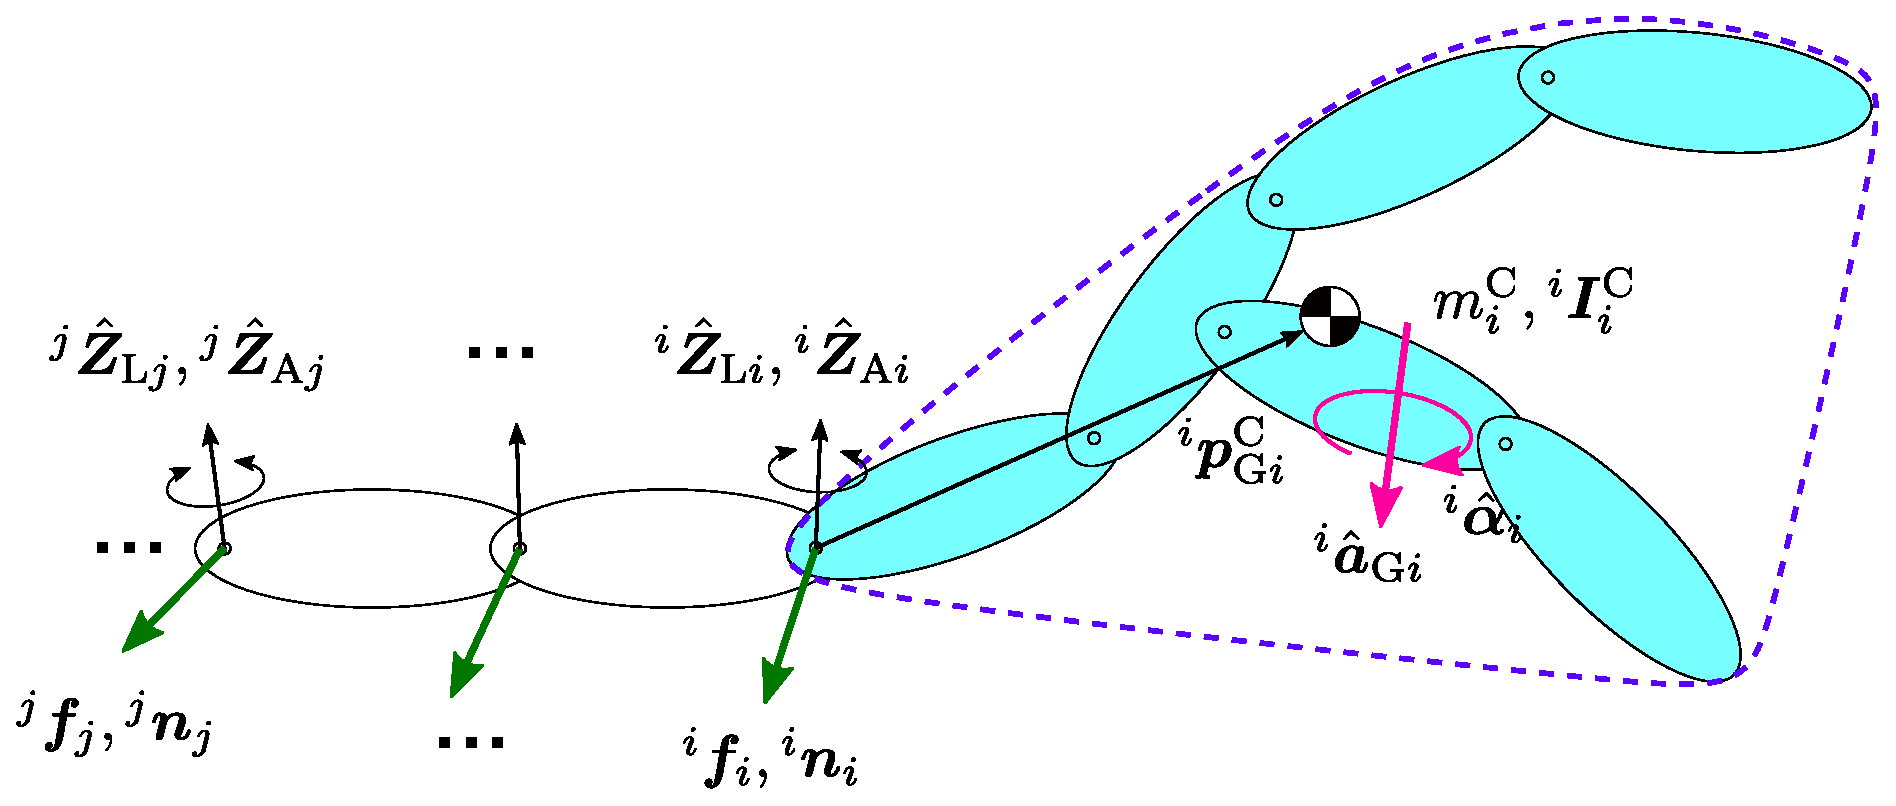
\includegraphics[width=.7\textwidth]{crb_force.eps}
\end{center}
\end{figure}

以上をまとめると,次式を得ます.
\begin{align*}
\left[\begin{array}{cc}
{}^{i}\hat{\bm{Z}}_{\mathrm{L}i}^{\mathrm{T}}
&
{}^{i}\hat{\bm{Z}}_{\mathrm{A}i}^{\mathrm{T}}
\end{array}\right]
\left[\begin{array}{cc}
{}^{j}\bm{R}_{i} & \bm{O}
\\
{}^{j}\bm{p}_{i}\times{}^{j}\bm{R}_{i} & {}^{j}\bm{R}_{j}
\end{array}\right]
\left[\begin{array}{cc}
m_{i}^{\mathrm{C}}\bm{1} & -m_{i}^{\mathrm{C}}{}^{i}\bm{p}_{\mathrm{G}i}^{\mathrm{C}}\times \\
m_{i}^{\mathrm{C}}{}^{i}\bm{p}_{\mathrm{G}i}^{\mathrm{C}}\times & {}^{i}\bm{I}_{i}^{\mathrm{C}}-m_{i}^{\mathrm{C}}{}^{i}\bm{p}_{\mathrm{G}i}^{\mathrm{C}}\times^{2}
\end{array}\right]
\left[\begin{array}{c}
{}^{i}\hat{\bm{Z}}_{\mathrm{L}i}
\\
{}^{i}\hat{\bm{Z}}_{\mathrm{A}i}
\end{array}\right]
\ddot{\bm{q}}_{i}
=
\bm{\tau}_{j}
\end{align*}
すなわち
\begin{align*}
\bm{H}_{ji}=
\left[\begin{array}{cc}
{}^{i}\hat{\bm{Z}}_{\mathrm{L}i}^{\mathrm{T}}
&
{}^{i}\hat{\bm{Z}}_{\mathrm{A}i}^{\mathrm{T}}
\end{array}\right]
\left[\begin{array}{cc}
{}^{j}\bm{R}_{i} & \bm{O}
\\
{}^{j}\bm{p}_{i}\times{}^{j}\bm{R}_{i} & {}^{j}\bm{R}_{j}
\end{array}\right]
\left[\begin{array}{cc}
m_{i}^{\mathrm{C}}\bm{1} & -m_{i}^{\mathrm{C}}{}^{i}\bm{p}_{\mathrm{G}i}^{\mathrm{C}}\times \\
m_{i}^{\mathrm{C}}{}^{i}\bm{p}_{\mathrm{G}i}^{\mathrm{C}}\times & {}^{i}\bm{I}_{i}^{\mathrm{C}}-m_{i}^{\mathrm{C}}{}^{i}\bm{p}_{\mathrm{G}i}^{\mathrm{C}}\times^{2}
\end{array}\right]
\left[\begin{array}{c}
{}^{i}\hat{\bm{Z}}_{\mathrm{L}i}
\\
{}^{i}\hat{\bm{Z}}_{\mathrm{A}i}
\end{array}\right]
\end{align*}
です.
ただし,$j$番目リンクが$i$番目関節よりも根元側にあることを前提としています.
$j$番目リンクが$i$番目リンクの属する枝と異なる枝にある場合はゼロ行列となります.
アルゴリズム上は,
\begin{align*}
\left[\begin{array}{c}
{}^{i}\hat{\bm{f}}_{i}
\\
{}^{i}\hat{\bm{n}}_{i}
\end{array}\right]
=
\left[\begin{array}{cc}
m_{i}^{\mathrm{C}}\bm{1} & -m_{i}^{\mathrm{C}}{}^{i}\bm{p}_{\mathrm{G}i}^{\mathrm{C}}\times \\
m_{i}^{\mathrm{C}}{}^{i}\bm{p}_{\mathrm{G}i}^{\mathrm{C}}\times & {}^{i}\bm{I}_{i}^{\mathrm{C}}-m_{i}^{\mathrm{C}}{}^{i}\bm{p}_{\mathrm{G}i}^{\mathrm{C}}\times^{2}
\end{array}\right]
\left[\begin{array}{c}
{}^{i}\hat{\bm{Z}}_{\mathrm{L}i}
\\
{}^{i}\hat{\bm{Z}}_{\mathrm{A}i}
\end{array}\right]
\\
\bm{H}_{ii}=
\left[\begin{array}{cc}
{}^{i}\hat{\bm{Z}}_{\mathrm{L}i}^{\mathrm{T}} &
{}^{i}\hat{\bm{Z}}_{\mathrm{A}i}^{\mathrm{T}}
\end{array}\right]
\left[\begin{array}{c}
{}^{i}\hat{\bm{f}}_{i}
\\
{}^{i}\hat{\bm{n}}_{i}
\end{array}\right]
\end{align*}
を先に計算しておき,
$i$番目リンクから親側にリンクをたどりながら,
\begin{align*}
{}^{i}\bm{S}_{j}=
\left[\begin{array}{cc}
{}^{i}\bm{R}_{j} & {}^{i}\bm{p}_{j}\times{}^{i}\bm{R}_{j}
\\
\bm{O} & {}^{i}\bm{R}_{j}
\end{array}\right]
\left[\begin{array}{c}
{}^{j}\hat{\bm{Z}}_{\mathrm{L}j}
\\
{}^{j}\hat{\bm{Z}}_{\mathrm{A}j}
\end{array}\right]
\\
\bm{H}_{ji}=
{}^{i}\bm{S}_{j}^{\mathrm{T}}
\left[\begin{array}{c}
{}^{i}\hat{\bm{f}}_{i}
\\
{}^{i}\hat{\bm{n}}_{i}
\end{array}\right]
\\
\bm{H}_{ij}=\bm{H}_{ji}^{\mathrm{T}}
\end{align*}
を求めていくのが良いでしょう.

\begin{figure}[h]
\begin{center}
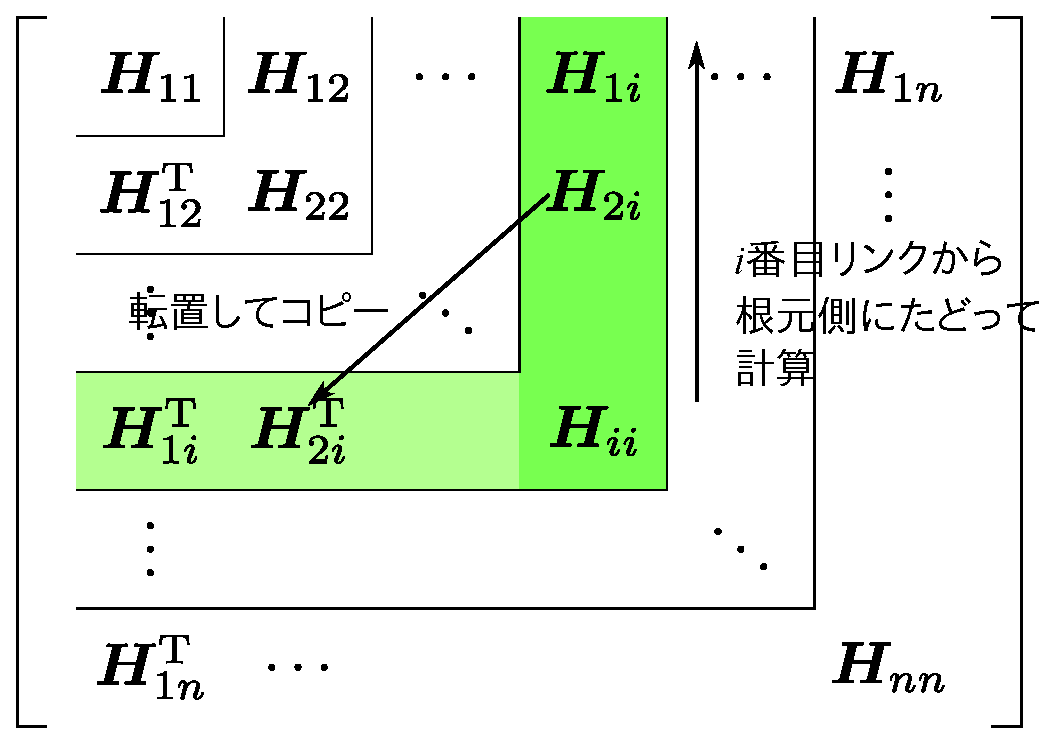
\includegraphics[width=.4\textwidth]{crb_mat_order.eps}
\end{center}
\end{figure}


\subsection{合成剛体の質量特性計算アルゴリズム}

$i$番目リンク座標系に対する
$i$番目合成剛体の質量$m_{i}^{\mathrm{C}}$,
重心位置${}^{i}\bm{p}_{\mathrm{G}i}^{\mathrm{C}}$,
慣性テンソル${}^{i}\bm{I}_{i}^{\mathrm{C}}$が計算できれば情報が揃います.
これらは再帰的に計算することが出来ます.

まず,$i$番目リンクが開リンク系の末端ならば,
\begin{align*}
m_{i}^{\mathrm{C}}=m_{i} \\
{}^{i}\bm{p}_{\mathrm{G}i}^{\mathrm{C}}={}^{i}\bm{p}_{\mathrm{G}i} \\
{}^{i}\bm{I}_{i}^{\mathrm{C}}={}^{i}\bm{I}_{i}
\end{align*}
です.
これらから根元側にさかのぼりながら,
\begin{align*}
m_{i}^{\mathrm{C}}=m_{i}+\sum_{j\in\mathcal{I}_{\mathrm{C}i}}m_{j}^{\mathrm{C}} \\
{}^{i}\bm{p}_{\mathrm{G}j}^{\mathrm{C}}={}^{i}\bm{p}_{j}+{}^{i}\bm{R}_{j}{}^{j}\bm{p}_{\mathrm{G}j}^{\mathrm{C}}
\\
{}^{i}\bm{p}_{\mathrm{G}i}^{\mathrm{C}}=
\left(
m_{i}{}^{i}\bm{p}_{\mathrm{G}i}+
\sum_{j\in\mathcal{I}_{\mathrm{C}i}}m_{j}^{\mathrm{C}}{}^{i}\bm{p}_{\mathrm{G}j}^{\mathrm{C}}
\right)\Big/
m_{i}^{\mathrm{C}}
 \\
{}^{i}\bm{I}_{i}^{\mathrm{C}}={}^{i}\bm{I}_{i}-m_{i}({}^{i}\bm{p}_{\mathrm{G}i}-{}^{i}\bm{p}_{\mathrm{G}i}^{\mathrm{C}})\times^{2}+
\sum_{j\in\mathcal{I}_{\mathrm{C}i}}\left\{
{}^{i}\bm{R}_{j}{}^{j}\bm{I}_{j}^{\mathrm{C}}{}^{i}\bm{R}_{j}^{\mathrm{T}}+
m_{j}^{\mathrm{C}}
({}^{i}\bm{p}_{\mathrm{G}j}^{\mathrm{C}}-{}^{i}\bm{p}_{\mathrm{G}i}^{\mathrm{C}})\times^{2}
\right\}
\end{align*}
と計算していけば良いです.
ただし,$\mathcal{I}_{\mathrm{C}i}$は$i$番目リンクの子リンクインデックス群です.
これらのうち$m_{i}^{\mathrm{C}}$は運動学情報を用いませんので,
最初に一度だけ計算して求めておけば良いことにご注意下さい.


\begin{figure}[h]
\begin{center}
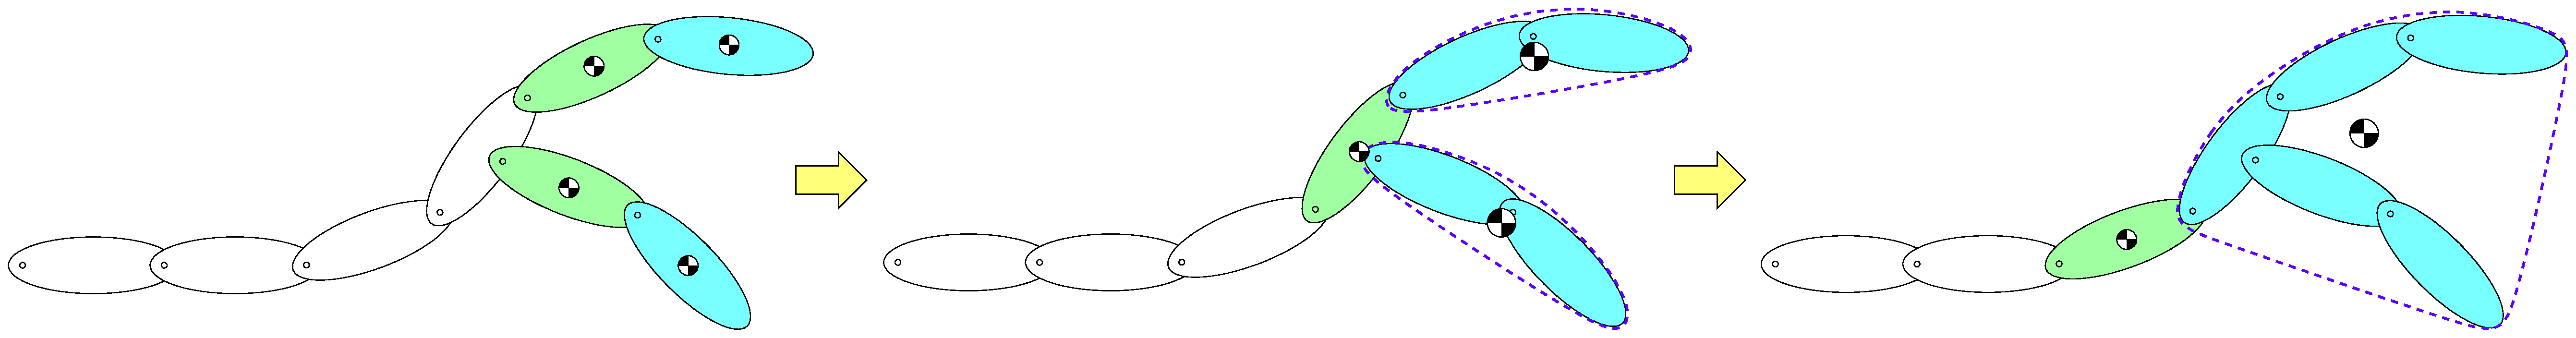
\includegraphics[width=\textwidth]{crb_building_process.eps}
\end{center}
\end{figure}


\subsection{RoKiでの実装}

RoKiでは合成剛体法を次の二つの関数で実装しています.
\begin{verbatim}
/* compute a cell of the inertia matrix of a kinematic chain based on the composite rigid body method. */
static void _rkChainLinkInertiaMatCRB(rkLink *link, zVec6D wi[], zVec6D si[], zMat hij, zMat inertia)
{
  rkLink *lp;
  zFrame3D f;
  int i, j;

  /* diagonal block */
  rkJointCRBWrench( rkLinkJoint(link), rkLinkCRB(link), wi );
  rkJointCRBXform( rkLinkJoint(link), ZFRAME3DIDENT, si );
  zMatSetSizeNC( hij, rkLinkJointSize(link), rkLinkJointSize(link) );
  for( i=0; i<rkLinkJointSize(link); i++ )
    for( j=0; j<rkLinkJointSize(link); j++ )
      zMatElemNC(hij,i,j) = zVec6DInnerProd( &si[i], &wi[j] );
  zMatPutNC( inertia, rkLinkJointIDOffset(link), rkLinkJointIDOffset(link), hij );
  /* non-diagonal block */
  for( lp=rkLinkParent(link); lp; lp=rkLinkParent(lp) ){
    _zFrame3DXform( rkLinkWldFrame(link), rkLinkWldFrame(lp), &f );
    rkJointCRBXform( rkLinkJoint(lp), &f, si );
    zMatSetSizeNC( hij, rkLinkJointSize(lp), rkLinkJointSize(link) );
    for( i=0; i<rkLinkJointSize(lp); i++ )
      for( j=0; j<rkLinkJointSize(link); j++ )
        zMatElemNC(hij,i,j) = zVec6DInnerProd( &si[i], &wi[j] );
    zMatPutNC(  inertia, rkLinkJointIDOffset(lp), rkLinkJointIDOffset(link), hij );
    zMatTPutNC( inertia, rkLinkJointIDOffset(link), rkLinkJointIDOffset(lp), hij );
  }

  if( rkLinkChild(link) )
    _rkChainLinkInertiaMatCRB( rkLinkChild(link), wi, si, hij, inertia );
  if( rkLinkSibl(link) )
    _rkChainLinkInertiaMatCRB( rkLinkSibl(link), wi, si, hij, inertia );
}

/* compute the inertia matrix of a kinematic chain based on the composite rigid body method. */
bool rkChainInertiaMatCRB(rkChain *chain, zMat inertia)
{
  zMatStruct hij;
  zVec6D wi[6], si[6];
  double _e[36];

  rkChainUpdateCRB( chain );
  zMatBufNC(&hij) = _e;
  _rkChainLinkInertiaMatCRB( rkChainRoot(chain), wi, si, &hij, inertia );
  return true;
}
\end{verbatim}

\verb|rkJointCRBWrench()|は${}^{i}\hat{\bm{f}}_{i}$および${}^{i}\hat{\bm{n}}_{i}$,
\verb|rkJointCRBXform()|は${}^{i}\bm{S}_{j}$を,
それぞれ求める関数です.
これは仮想関数で,実体は各関節クラスのメンバ関数として個別に実装することで高速化しています.
関節クラスには
固定関節(fixed),
回転関節(revolute),
直動関節(prismatic),
円筒関節(cylindrical),
自在継手(ユニバーサル関節 Hooke),
球面関節(spherical),
浮遊関節(float)を用意してあります.

$m_{i}^{\mathrm{C}}$の再帰的計算は\verb|rkLinkUpdateCRBMass()|,
${}^{i}\bm{p}_{\mathrm{G}i}^{\mathrm{C}}$および${}^{i}\bm{I}_{i}^{\mathrm{C}}$の再帰的計算は
\verb|rkLinkUpdateCRB()|でそれぞれ実装しています.

慣性行列の計算は,
\begin{itemize}
\item \verb|rkChainInertiaMatCRB()|(合成剛体法)
\item \verb|rkChainInertiaMatUV()|(単位ベクトル法)
\item \verb|rkChainInertiaMatMJ()|(ヤコビ行列を用いて直接的に求める方法)
\end{itemize}
を実装していますが,
合成剛体法の計算時間は他の二つの計算時間の半分程度のようです.


\end{document}
